\input templates/header
\title[DS - Models]{\textbf{Distributed Algorithms}\\Models}

\begin{document}


\begin{frame}
\titlepage
\end{frame}

\section{Taxonomy}


\begin{frame}{Taxonomy of Distributed Systems}
Architectures:
\BI
\item Client-server
\item Multi-tier
\item Clusters
\item Cloud computing
\item Peer-to-Peer
\item Sensor networks $\rightarrow$ See companion course
\EI
\end{frame}

\subsection{Client-server}

\begin{frame}{Client-server}
\begin{columns} 
\begin{column}{0.65\textwidth} 
\BI
\item The easiest form of distributed systems
\bigskip
\item Resources are centralized on servers
\bigskip
\item Large number of clients access them through request-reply interactions
\bigskip
\EI
\end{column}
\begin{column}[c]{0.35\textwidth}
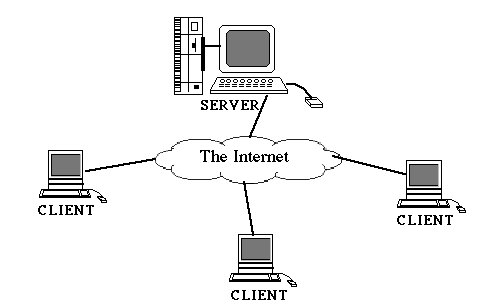
\includegraphics[width=\textwidth]{figs/01/client-server.png}
\end{column}
\end{columns}

\end{frame}

\begin{frame}[shrink]{Client-server: problem examples}
\begin{block}{Reliable message delivery}
TCP/IP: Guarantee the delivery of message in FIFO order
\end{block}

\begin{block}{Resource lease}
DHCP: Lend limited resources for a predefined period of time
\end{block}

\begin{block}{Remote procedure call}
Allow invocation of procedures/methods/functions on remote objects
\BI
\item RPC ('60)
\item CORBA ('90)
\item Java RMI, .Net WCF 
\item JSON-RPC, XML-RPC
\item Google Protocol Buffers, Apache Thrift, Apache Avro, Twitter Finagle
\EI
\end{block}

\end{frame}



\subsection{Multi-tier}

\begin{frame}{Multi-tier}
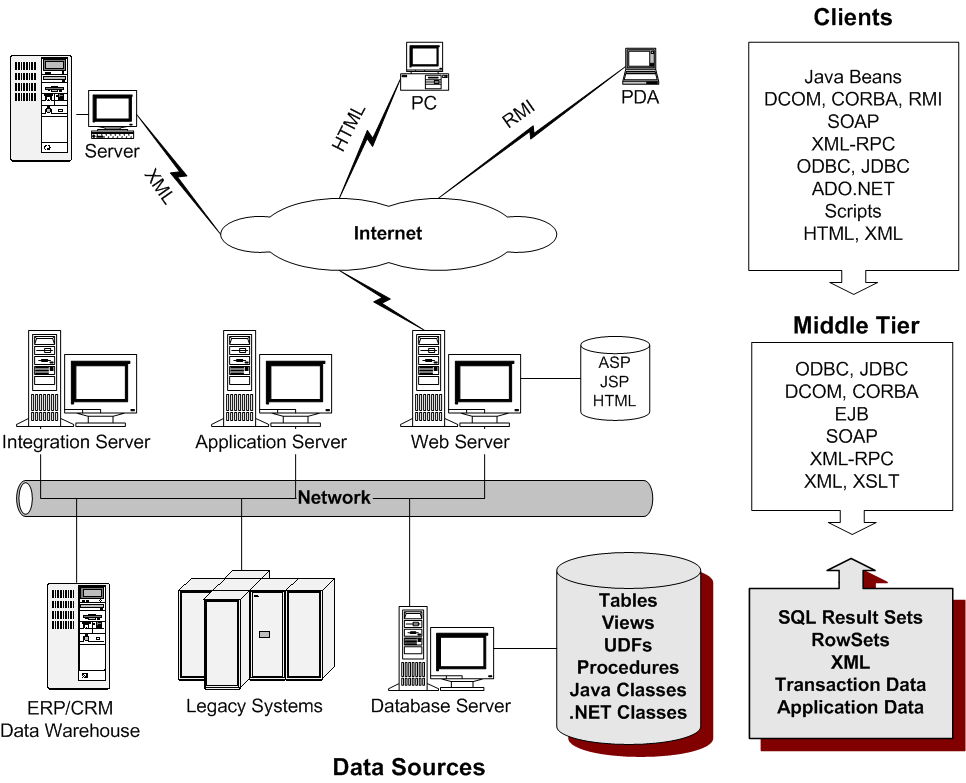
\includegraphics[width=0.8\textwidth]{figs/01/multi-tier.png}	
\end{frame}

\begin{frame}{Multi-tier: problem examples}
	
\begin{block}{Total order broadcast}
Processes may not only to agree on which actions they should execute...\\
But also in the order in which they are executed
\end{block}

\bigskip
Example
\BI
\item Initial state: Process $A$: $c=1$, Process $B$: $c=1$
\item Process $A$: [$c \gets c \cdot 3$] [$c \gets c+1$]
\item Process $B$: [$c \gets c+1$] [$c \gets c \cdot 3$]
\item Inconsistency! 
\EI
\end{frame}

\subsection{Cluster computing}

\begin{frame}{Cluster computing}
	
\BI
\item A group of high-end systems connected through a fast LAN
\item Homogeneous: same OS, near-identical hardware
\item Single managing node
\item Example: Mosix/OpenMosix
\EI

\begin{figure}
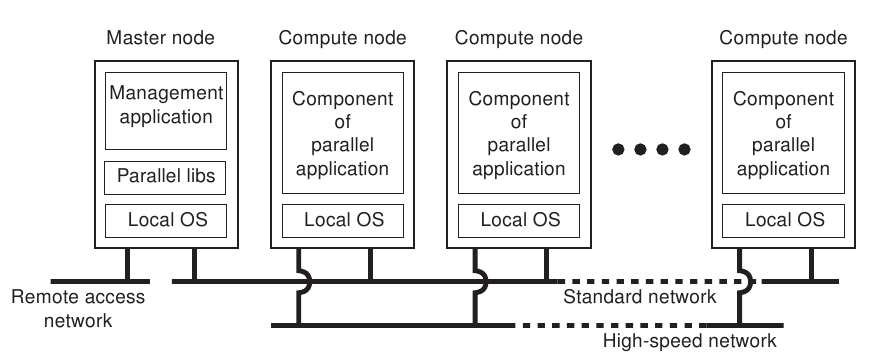
\includegraphics[width=\textwidth]{figs/01/cluster.png}	
\end{figure}

\end{frame}

\begin{frame}{Cluster computing: problem examples}

\begin{block}{Load balancing}
\BI
\item Different nodes may be subject to different computational load
\item Possible techniques for load balancing:
  \BI
  \item Assign new tasks to under-loaded nodes
  \item Migrate tasks from overloaded nodes to underloaded nodes
  \EI
\EI

\end{block}

\begin{block}{Message passing / synchronization}
\BI
\item PVM, the Parallel Virtual Machine
\BI
\item provides a run-time environment for message-passing, task and resource management, and fault notification
\EI
\item MPI, the Message Passing Interface
\BI
\item a standardized and portable message-passing system designed by a group of researchers from academia and industry to function on a wide variety of parallel computers
\EI
\EI
\end{block}

\end{frame}

\subsection{Cloud computing}

\begin{frame}{Cloud computing}

\begin{block}{Informal definition}	
Cloud computing is a general term that describes a new class of network-based 
computing taking place over the Internet (\alert{utility computing})
\end{block}
\medskip
\BI
\item A collection/group of integrated and networked hardware, software and Internet infrastructure (called a platform).
\item Using the Internet for communication and transport provides hardware, software and networking services to clients.
\item These platforms hide the complexity and details of the underlying infrastructure from users and applications by 
providing graphical interfaces or API
\EI
\end{frame}

\begin{frame}{Different cloud computing layers}
\BI
\item Software as a service (SaaS)
\item Platform as a service (PaaS)
\item Infrastructure as a service (IaaS)
\EI

\begin{figure}
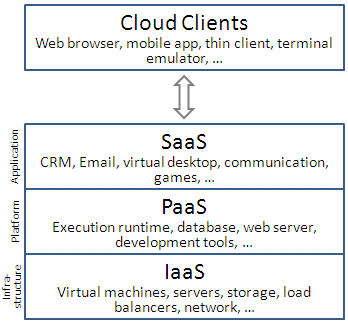
\includegraphics[width=0.5\textwidth]{figs/02/cloud_computing_layers.png}	
\caption{Source: Wikipedia}
\end{figure}


\end{frame}

\begin{frame}{An example: Amazon}

{\footnotesize 
\begin{columns}
\begin{column}{0.50\textwidth}
\BI
\item Compute\\
-- Elastic Compute Cloud (EC2)\\
-- Elastic MapReduce\\
-- Auto Scaling

\item Content Delivery\\
-- CloudFront\\

\item Database\\
-- DynamoDB\\
-- Relational DB Service (RDS)

\item E-Commerce\\
-- Fulfillment Web Service (FWS)

\item Messaging\\
-- Simple Queue Service (SQS)\\
-- Simple Notification Service (SNS)
\EI
\end{column}
\begin{column}{0.50\textwidth}
\BI
\item Monitoring \\
-- CloudWatch

\item Networking\\
-- Virtual Private Cloud (VPC)\\
-- Elastic Load Balancing

\item Payments \& Billing \\
-- Flexible Payments Service (FPS) \\
-- DevPay

\item Storage\\
-- Simple Storage Service (S3) \\
-- Elastic Block Storage (EBS) \\
-- AWS Import/Export

\EI

\end{column}
\end{columns}
}

\end{frame}

\subsection{Peer-to-peer systems}

\begin{frame}{Peer-to-peer}
\begin{block}{Definition}
A peer-to-peer system is a collection of peer nodes  \\
Each peer is both a server and a client (“servent”)
\BI
\item Provides resources to other peers
\item Consumes resources from other peers
\EI
\end{block}

\bigskip
Characteristics:
\BI
\item Put together resources at the edge of the Internet
\item Share resources by direct exchange between nodes
\item Perform critical functions in a decentralized manner
\EI
\end{frame}

\begin{frame}{Overlay networks}
\begin{figure}
	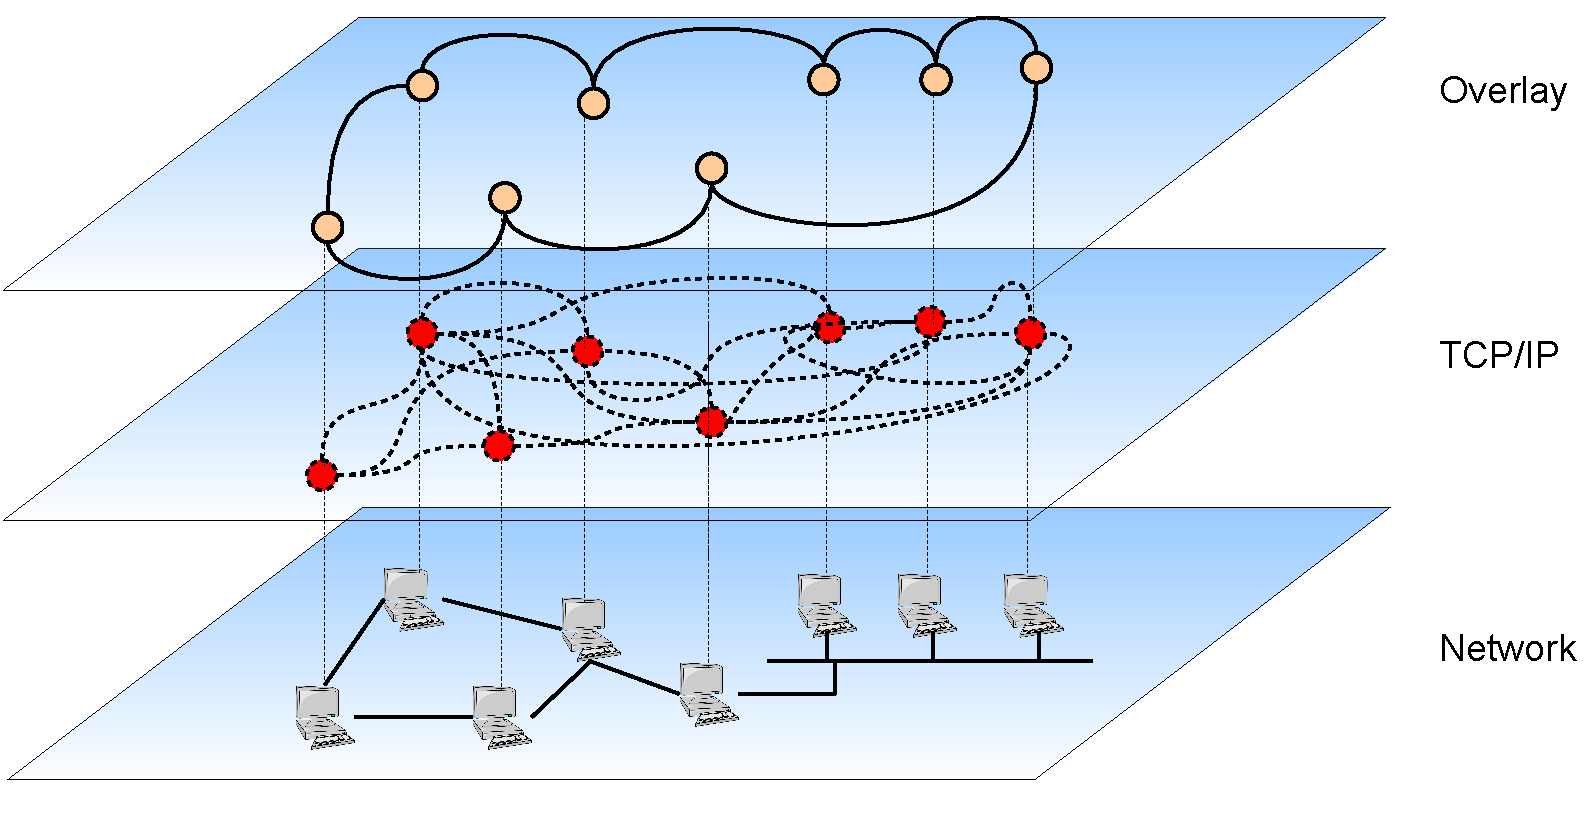
\includegraphics[width=\textwidth]{figs/10/overlay}
\end{figure}
\end{frame}

\begin{frame}{Peer-to-peer systems: problem examples}

\begin{block}{P2P key-value stores}
A peer-to-peer service that offers an associative \alert{Map} interface:
\BI
\item \alert{$\mathit{put}(\textsc{Key}\ k,\ \textsc{Value}\ v)$}: associate a value $v$ to the key $k$
\item \alert{$\textsc{Value}\ \mathit{get}(\textsc{Key}\ k)$}: returns the value associated to key $k$
\EI
\end{block}

\medskip
\structure{(Distributed) Hash Tables}:\\
\BI
\item Hash tables map keys to memory locations
\item Distributed hash tables map keys to nodes
\EI

\medskip
\structure{Organization}:\\
\BI
\item Each node is responsible for a portion of the key space
\item Messages are routed between nodes to reach responsible nodes
\item Replication used to tolerate failures
\EI

\end{frame}

\begin{frame}{Routing in DHTs}

\begin{figure}
	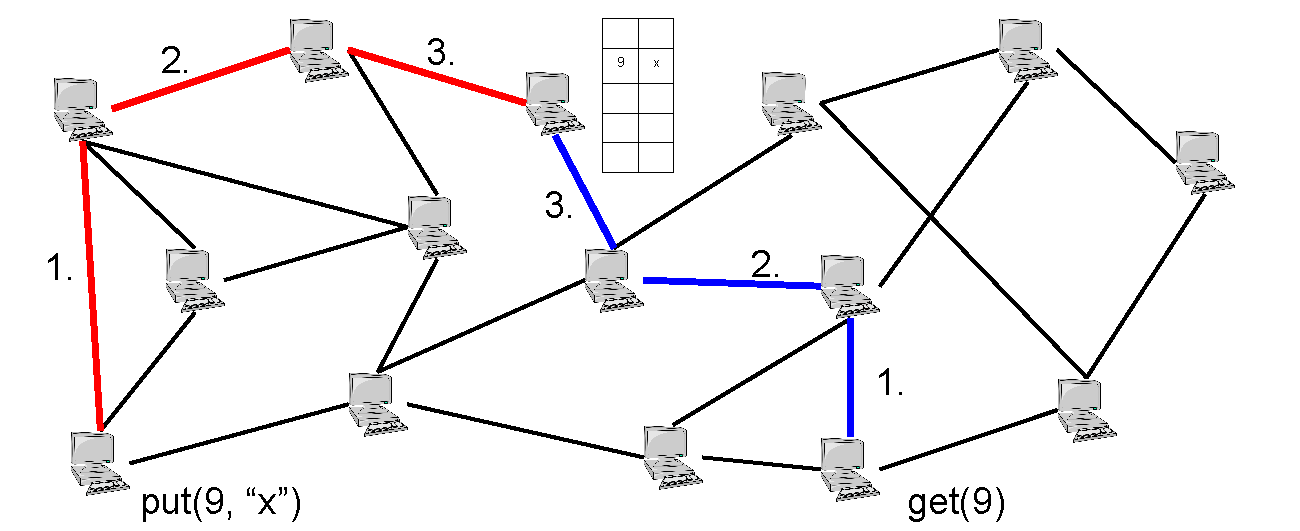
\includegraphics[width=\textwidth]{figs/10/dht-routing}
\end{figure}

\end{frame}


\section{Modeling Distributed Systems}


\begin{frame}{Contents}

\structure{Modeling distributed systems}
\BIL
\item \alert{Computation}:
  Processes, deterministic vs probabilistic behavior
\item \alert{Interaction}: 
  Processes interact through \highlight{messages}, which result in:
  \BI
    \item Communication, i.e. information flow
    \item Coordination, i.e. synchronization and ordering of activities
  \EI
\item \alert{Failures}:
  Which kind of failures can occur?
  \BI 
  \item Benign vs malicious (Byzantine)
  \item Process vs communication
  \EI
\item \alert{Time}:
  Determining whether we can make any assumption on time bounds
  on communication and computation speeds.
\EIL

\end{frame}



\subsection{Computation}

\begin{frame}{Computation}

\BIL
\item \alert{Process}: the unit of computation in a distributed system.\\
Sometimes we may call it node, host, etc. 
\item \alert{Process set}: denoted by $\Pi$, it is composed by a 
collection of $n$ uniquely identified processes, like 
$p_1, p_2, \ldots, p_n$.
\item Typical assumptions:
  \BI
  \item The set is static ($n$ is well-defined);
  \item Processes do know each other
  \item All processes run a copy of the same algorithm; the sum of
    all these copies constitutes the distributed algorithm
  \EI
\item But in extreme distributed systems:
  \BI
  \item Dynamic set
  \item Too many, too dynamic to know them all
  \item Multiple algorithms
  \EI
\EIL
\end{frame}



\begin{frame}{Deterministic vs probabilistic}

\BIL
\item \alert{Deterministic process}: the local computation and the messages
  sent by a process is determined by the current state and the messages 
  previously received.
\item \alert{Probabilistic process}: processes may make used of \alert{random}
  oracles to choose the local computation to be performed or the next
  message to be sent.
\EIL

\end{frame}

\subsection{Interaction}

\begin{frame}{Interaction}
\note{
\BI
\item In the receive operation, we do not specify the original sender;
  can be
\item Fully connected topology may be obtained through routing. For
  example, consider the following architectures:
  \BI
  \item Fully connected mesh
  \item broadcast medium (Ethernet, wireless)
  \item Ring
  \item ``Internet'' with routers
  \EI
\EI
}	
	
	
\BIL
\item Processes communicate through \highlight{messages}
  \BI 
  \item $\send(m,p)$: sends a message $m$ to $p$
  \item $\receive(m)$: receives a messages $m$ 
  \EI
\item In some cases, messages may be uniquely identified by
  \BI 
  \item Sender of the message
  \item A sequence number local to the sender
  \EI
\item General assumption: every pair of processes is connected by a bi-directional \alert{communication channel}
\BI
\item Through routing
\item Not true for P2P systems
\EI
\EIL
\end{frame}

\subsection{Failures}

\begin{frame}{Process failures}

In a distributed systems, both processes and communication channels may fail, i.e. depart from
what is considered its correct behavior.\\
Hadzilacos and Toueg~\cite{hadzilacos94modular} provide a taxonomy. 

\begin{block}{Benign process failures}
\BI
\item \alert{Fail-stop}: A process stops executing events, and other processes may detect this fact.
\item \alert{Crash}: A process stops executing events
\EI
\end{block}

\begin{block}{Malicious process failures}
\BI
\item \alert{Arbitrary failure}, or Byzantine: any type of error may occur. This may be caused by:
  \BI
  \item A software bug
  \item A malicious behavior inspired by an intelligent adversary
  \EI
\EI
\end{block}

\end{frame}

\begin{frame}{Process failures}
	
\note{
To avoid the problem of amnesia completely, every read/write would have to pass
through permanent memory; too expensive
}

\BIL
\item A process that never fails is \alert{correct}
\item A process that eventually fails is \alert{faulty}
\item Several protocols are designed to work correctly if the number
  of failures $f$ is bounded (for example, $f < n/3$).
\item In some models, processes may perform a \highlight{recovery} action:
  \BI
  \item After some time, a process may resume functioning
  \item It suffers {\em amnesia}: the local state maintained in volatile
    memory is lost
  \item To limit the effects of amnesia, a log can be maintained
 \EI
\EIL

\end{frame}

\begin{frame}{Communication failures}

\begin{block}{Benign communication failures}
\BI
\item Process $p$ performs {\tt send} of a message $m$ to process $q$
\item Message $m$ is inserted in a local outgoing buffer of $p$ (\alert{Send-omission})
\item Message $m$ is transmitted from $p$ to $q$ (\alert{Omission})
\item Message $m$ is inserted in a local incoming buffer of $q$ (\alert{Receive-omission}) 
\item Process $q$ performs {\tt receive} of $m$
\EI
\end{block}

\begin{block}{Malign communication failures}
Messages created out of nothing, duplicated messages, etc. \\
These problems can easily be solved through encryption techniques.
\end{block}

\end{frame}

\begin{frame}{Communication failures}

Possible causes of message failures:
\BIL
  \item \alert{Buffer overflow} in the operating system
  \item \alert{Congestion}, routing errors in routers
  \item \alert{Partitioning}:
    \BI
    \item Processes are subdivided in disjoint sets called \alert{partitions}
    \item Communication inside a partition is possible
    \item Communication between partitions is not possible
    \EI
    When a partition disappears, we say that partitions {\em merge}
\EIL
\end{frame}

%\subsection{Communication channels}

\begin{frame}{Modeling (faulty) communication channels}

The idea: the channels cannot systematically drop a specific message. This is the minimum abstraction
needed to create reliable channels.

\bigskip
\begin{block}{Fair-Loss Channels}
	
\BIL
\item \alert{ Validity -- Fair Loss}: If a message $m$ is sent infinitely often by a process $p$ to a process $q$ and
  neither $p$ and $q$ crash, then $q$ will receive $m$ infinitely often
\item \alert{Integrity -- Finite Duplication}: If a message $m$ is sent a finite number of times by a process $p$ to
a process $q$, then $m$ cannot be received by $q$ an infinite number of times
\item \alert{Integrity -- No creation}: If a message $m$ is delivered by some process $p$, then $m$ was previously sent
by some process $q$ to $p$
\EIL

\end{block}


\end{frame}

\begin{frame}{Modeling (correct) communication channels}

The idea: channels are reliable, messages are never lost. It can be implemented, but 
there is a price to be payed: asynchrony.

\bigskip
\begin{block}{Perfect Channels}

\BIL
\item \alert{Validity -- Reliable delivery}: If $p$ sends a message to $q$, and neither of $p$ and $q$ crash, then 
$q$ will \alert{eventually} receive $m$
\item \alert{Integrity -- No duplication}: No message is delivered to a process more than once
\item \alert{Integrity -- No creation}: If a message $m$ is delivered by some process $p$, then $m$ was previously sent
by some process $q$ to $p$
\EIL

\end{block}


\end{frame}


\begin{frame}[shrink=16]{An Example Algorithm}

\begin{Procedure}
\caption{Fair-loss Channel $\rightarrow$ Perfect Channel} 
\UPON{\Init}{
  $\Set\ \Sent \gets \emptyset$\;
  $\Set\ \Delivered \gets \emptyset$\;
  $\textsf{startTimer}(\Timeout)$\;
}
\UPON{\Timeout}{
  \ForEach{$(m,q) \in \Sent$}{
    $\FairLossSend(m,q)$\;
  	$\textsf{startTimer}(\Timeout)$\;
  }
}
\UPON{$\PerfectSend(m,q)$}{
  $\FairLossSend(m,q)$\;
  $\Sent \gets \Sent \cup \{ (m,q) \}$\;
}
\UPON{$\FairLossReceive(m,q)$}{
  \If{$m \notin \Delivered$}{
    $\Delivered \gets \Delivered \cup \{ m \}$\;
    $\PerfectReceive(m,q)$\;
  }
}
\end{Procedure}

\end{frame}

\begin{frame}{Safety and liveness}
\begin{block}{Safety}
\begin{quote}	
``Something bad will never happen''
\end{quote}
  In other words, a distributed program should never enter an
  unacceptable state.
  \BI
  \item No message is delivered to a process more than once.
  \EI
\end{block}

\begin{block}{Liveness}
\begin{quote}	
``Something good eventually does happen''
\end{quote}	

  In other words, a distributed program \alert{eventually} enters a desirable
  state.
  \BI
  \item If $p$ sends a message to $q$, and neither of $p$ and $q$ crash, then \alert{eventually}
$q$ will receive $m$.
  \EI
\end{block} 
\end{frame}

\subsection{Time}

\begin{frame}{Time}
\BIL
\item \alert{Global clock}
  \BI
  \item
  For presentation simplicity, it may be convenient to assume
  the presence of a {\em global real-time clock}, outside the control of processes.
  \item This can be used to provide a global ordering of steps in a distributed systems
  \EI
\item \alert{In reality}:
  \BI
  \item Each process is associated with a \alert{local clock}
  \item Local clocks may not report the perfect time
  \item \alert{Clock drift rate}: refers to the {\em relative} amount that a computer
    clock differs from a perfect reference clock.
  \EI
\item Synchronization is possible, but expensive:
  \BI
    \item Atomic clocks
    \item GPS
	\item See: Google TrueTime API:
  \EI
\EI

\note{
    \BI
      \item GPS does not work into buildings
      \item Atomic clocks: cost not justified
    \EI
}

\end{frame}

\begin{frame}{Time measures associated to communication}

\BIL
\item \alert{Latency}: The delay between the start of message sending from one process and the
  beginning of its receipt by another. Possible causes:
  \BI
   \item the actual time for bit transmission (e.g., satellite link)
   \item the delay for accessing the network, especially in case
     of congestion
   \item the time taken by the operating system to handle the message
     both at sender and receiver
  \EI
\item \alert{Bandwidth}: Total amount of information that can be transmitted
  over a communication channel in a given time. 
\item \alert{Jitter}: Variation in the time taken to deliver a series of
  messages. Mostly related with multimedia data.
\EIL
\end{frame}


\begin{frame}{Asynchronous vs synchronous}

\begin{block}{Distributed Systems vs Time}
Distributed systems make difficult to reason about time, not only for lack
of clock synchronization. It is also difficult to pose time bounds on 
events and communication.
\end{block}

\bigskip
We may think about several different models:
\BIL
\item \alert{Asynchronous} distributed systems 
\item \alert{Synchronous} distributed systems 
\item \alert{Partially synchronous} distributed systems
\EIL

\note{
\BI
\item \alert{Asynchronous} distributed systems 
  \BI
    \item No assumptions can be made.
    \item Most of the problems cannot be solved
  \EI
\item \alert{Synchronous} distributed systems 
  \BI
    \item Precise assumptions are possible on computation, communication time and
clocks.
   \item Not really realistic / difficult to implement
  \EI
\item \alert{Partially synchronous} distributed systems
  \BI
   \item Some assumptions can be made, others not, OR
   \item Assumptions can be made statistically, OR
   \item Assumptions hold for arbitrarily long periods of time
  \EI
\EI

}


\end{frame}

\begin{frame}{Asynchronous vs synchronous}

\begin{block}{Asynchronous distributed system}
\BI
\item There are no bounds on the relative speed of process execution.
\item There are no bounds on message transmission delays.
\item There are no bounds on clock drift.
\BI
\item OR, since we cannot count on their precision at all, {\em there are no clocks}.
\EI
\EI
\end{block}

\end{frame}

\begin{frame}{Asynchronous vs synchronous}

\structure{Comments}
\BIL
\item These are not assumptions! These are ``lack of assumptions''!
\item The worst possible model: services as simple as:
  \BI
  \item failure detection 
  \item time-based coordination
  \EI
  are not possible
\item Advantages:
 \BI
  \item simple semantics
  \item easier to port to more ``powerful'' models
  \item More realistic: several sources of asynchrony are present
    in a large-scale network (like the Internet)
  \EI
\EIL
\end{frame}

\begin{frame}{Asynchronous vs synchronous}

\begin{block}{Synchronous Distributed Systems }

\BI
\item {\em Synchronous computation}: \\
  There is a known upper bound on the relative speed of process execution.
\item {\em Synchronous communication}: \\
  There is a known upper bound on message transmission delays.
\item {\em Synchronous clocks}: \\
  Processes are equipped with local clocks. There is a known upper bound on
  the drift rates of local clocks with respect to a global real-time clock.
\EI
\end{block}

\end{frame}

\begin{frame}{Asynchronous vs synchronous}

\structure{Comments}
\BIL
\item The best possible model. Can be built, but not with standard hardware/software.
\BI
  \item Synchronous Ethernet vs CSMA/CD Ethernet
  \item Real-time OS vs normal OS
\EI
\item Many interesting properties:
  \BI
  \item Timed failure detection (e.g., ping)
  \item Coordination based on time (e.g., lease)
  \item Worst-case performance analysis
  \item Synchronized clocks
  \EI
\EIL

\end{frame}

\begin{frame}{Asynchronous vs synchronous}

\begin{block}{Partial synchrony}
For most systems we know of, it is relatively easy to define physical time bounds that
are respected {\em most of the time}. There are however periods where the timing assumptions
do not hold.
\end{block}

\BIL
\item Delays on processes:
\BI
\item Machines may run out of memory, slowing down processes
\item A typical case of {\em ``no bound on relative speeds of processes''}
\EI

\item Delays on messages:
\BI
\item Network may congested, and messages may be dropped.
\item Re-transmission protocols can ensure reliability, but at the price of asynchrony\\
  Messages may be re-transmitted an arbitrary number of times.
\EI
\EIL
\note{
In this sense, practical systems are {\em partially synchronous}
}

\end{frame}

\begin{frame}{Asynchronous vs synchronous}
	
How to express partial synchrony? A possibility is the following:
\begin{quote}
  Timing assumptions only hold \alert{eventually}.
\end{quote}
\alert{Theoretically, it means:}
\BI
\item There is a time after which the system is synchronous forever
\item The system is initially asynchronous and only after a long time becomes synchronous
\EI
\alert{How to read it:}
\BI
\item The system is not always synchronous
\item There is no known bound to the period in which it is asynchronous
\item We expect that there are periods during which the system is synchronous
\item Some of these periods are long enough to terminate protocol execution
\EI
\end{frame}

\section{Bibliography}

%\nocite{ozalp93consistent}

\begin{frame}{Reading material}

{\footnotesize
\bibliographystyle{abbrv}
\bibliography{references}  
}

\end{frame}


\end{document} 
